The Tritium-IFIC 2 prototype simulation was the last simulation carried out in TRITIUM experiment. It consists of $800$ fibers of $1~\mm$ diameter uniformly distributed in sixteen different circles of increasing radius, as illustrated in Figure \ref{fig:FibersTritiumIFIC2Simulation}. The optical properties were included.

\begin{figure}[h]
\centering
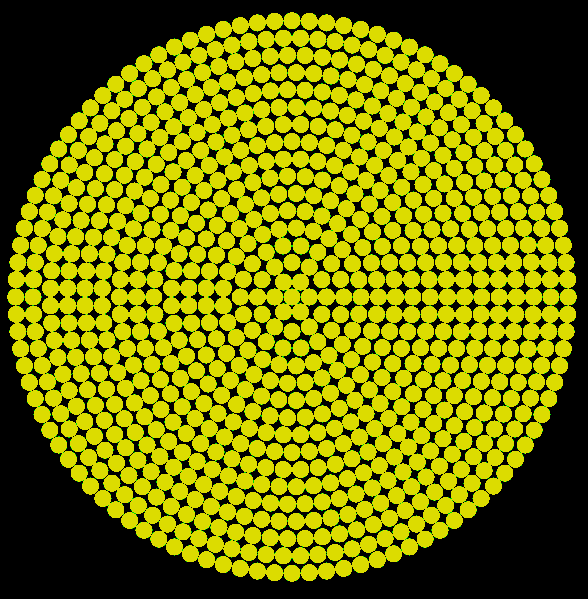
\includegraphics[scale=0.4]{6Simulations/64Tritium_IFIC_2/FiberDistribution_Tritium_IFIC_2_simulation.png}
\caption{Distribution of the scintillating fibers in the simualtion of Tritium-IFIC 2 prototype.\label{fig:FibersTritiumIFIC2Simulation}}
\end{figure}
The tritiated water source consists of a tritiated water volume with a thickness of $5~\mu\meter$ around each scintillating fiber. Scintillating fibers are located inside of a Teflon vessel, which was simulated with dimensions given above. Two PMMA windows of $5~\mm$ thickness located in both fiber ends and a optical grease layer with a thickness of $0.5~\mm$ located in each PMMA windows were included. Two PMTs, model R8520-460 from Hamamatsu \cite{DataSheetPMTs}, were also simulated as photosensors. 

%The optical properties used for the tritiated water, Teflon vessel, PMMA windows and the optical grease, mentioned in section \ref{sec:Geant4Environment}, are included in this simulation. 

The geometry simulated for TRITIUM-IFIC 2 is shown in Figure \ref{fig:TritiumIFIC2Simulation} in which is shown the PMTs (black), the optical grease (blue), PMMA windows (white), tritiated water (green) and scintillating fibers (yellow). In this image, the Teflon container is not drawn to allow its interior to be seen. Several volumes of tritiated water were also excluded to allow several scintillation fibers to be seen.

\begin{figure}[h]
\centering
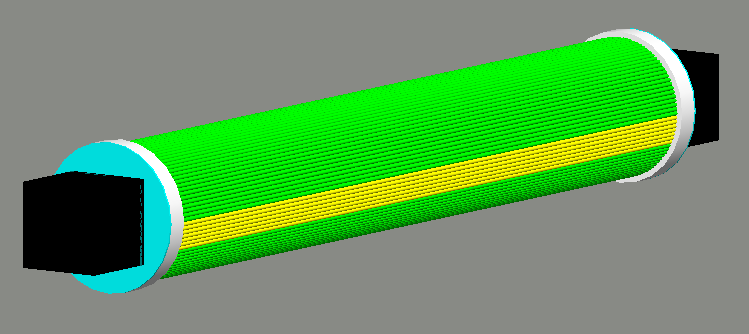
\includegraphics[scale=0.4]{6Simulations/64Tritium_IFIC_2/SimulationTritiumIFIC2.png}
\caption{Simualtion of Tritium-IFIC 2 prototype. PMTs (black), the optical grease (blue), PMMA windows (white), tritiated water (green) and scintillating fibers (yellow). \label{fig:TritiumIFIC2Simulation}}
\end{figure}

The used PMTs do not cover the entire active area formed by the scintillating fiber bundle. This is not a problem for the TRITIUM detector since its final version will use SiPM arrays.

The results obtained with the simulation of the TRITIUM-IFIC 2 prototype are shown in section \ref{subsec:ResultsSimulatedTRITIUMIFIC2}.


%The simulation of the Tritium-Aveiro prototype is similar to this since the design of both detectors are quite similar. There are two main difference between both simulated prototypes:

%\begin{enumerate}

%\item{} The diameter of the fibers used, which is $1~\mm$ for Tritium-IFIC 2 prototype and $2~\mm$ for Tritium-Aveiro prototype. As the internal volume of the Teflon vessel is filled, this difference imply a difference number of the scintillating fibers used, causing a difference in the signal-background ratio.

%\item{} The photosensors used since, although both are PMTs, the model of the used PMTs is different and it cause a different active area readout, affecting to the tritium detection efficiency. 

%\end{enumerate}